\section{Experimental evaluation}
\label{sec:evaluation}

We performed two types of evaluation: a first assessment done on the \textbf{working prototype} running on multiple Virtual Machines (VMs) and an evaluation using simulations run on a \textbf{discrete-event simulator}.
In the first case, since it's not possible to emulate a network similar to a real edge network due to the amount of resources needed, we focus on the \textbf{effectiveness}, \textbf{efficiency} and \textbf{usability} of the framework.
While with the discrete-event simulation at hand we can focus on the \textbf{latency} and the \textbf{bandwidth} consumed.


\subsection{Performance}
We found that, after paying the \textbf{cold-start} price where the initialization of the container running the function would create a noticeable latency, functions were executed in milliseconds even when using the (local) stateful support. This speed of the stateful support has been possible thanks to the usage of an in-memory database like Redis.

We also tested the \textbf{scalability} of our solution when using the \textit{faas} flavour of OpenFaas: we made 10'000 sequential calls to a node running a simple function and we noticed that new containers were immediately created to fulfill the stream of requests. After the 10'000 calls ended and no new calls were made, OpenFaas automatically scaled down and brought the number of idle containers to one.


\subsection{Usability}
We tested our solution with the implementation of some use cases.
Our solution allows developers to forget about the location, which instead is handled internally, and forget about handling the complex management of hundreds of geo-distributed nodes.
This avoids the creation of custom solutions that overfit on the available infrastructure, creating a code that becomes task-specific and difficult to extend and maintain.
In fact, developers would need to set up the infrastructure all by themselves, a process which can create errors or malfunctions, while the serverless FaaS architecture in our solution allows to forget about the handling of the infrastructure.

\subsection{Simulation Summary}
Thanks to the various experiments performed on the simulation, we found that by using our framework we get immense benefits in terms of \textbf{reduced traffic} in the network (Figure \ref{fig:write-by-traffic1}), while allowing \textbf{faster reads} when the data aggregation needed is not central.

\begin{figure}
    \centering
    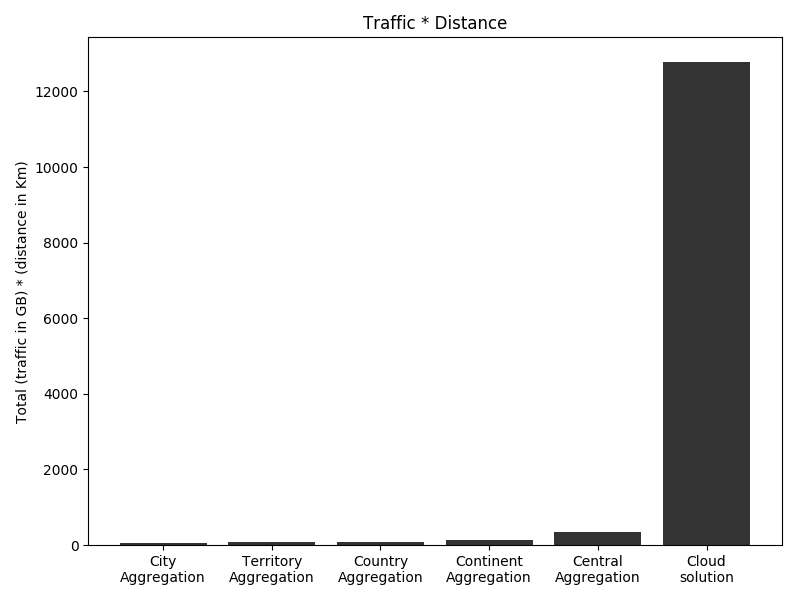
\includegraphics[width=0.99\linewidth]{Figures/Evaluation/write-by-traffic1-simplified.png}
    \caption{Traffic per distance generated in the network.}
    \label{fig:write-by-traffic1}
\end{figure}

\iffalse
\begin{figure}
    \centering
    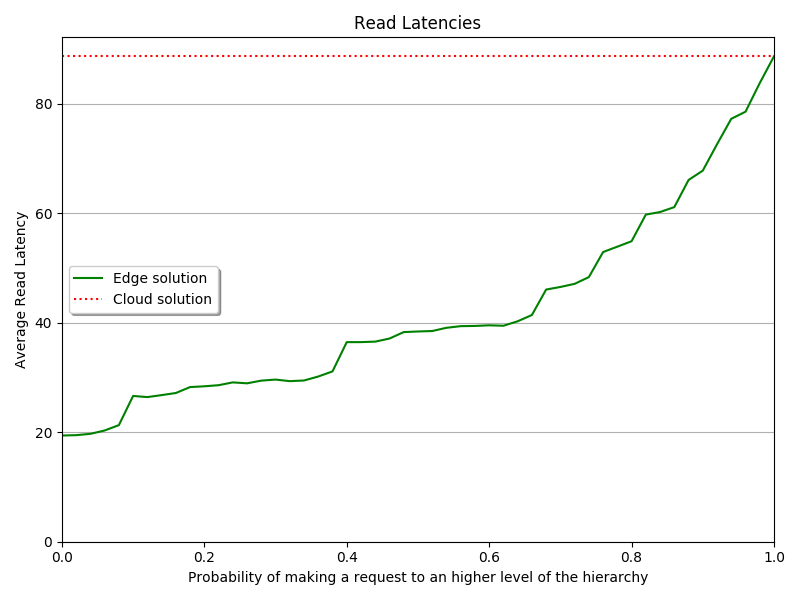
\includegraphics[width=0.99\linewidth]{Figures/Evaluation/read-all-latency.png}
    \caption{Average read latency as a function of the probability of making the read request to an higher level}
    \label{fig:read-all-latency}
\end{figure}
\fi

In a case where a central aggregation is still needed we found that the write requests suffer an increase in latency, but the increase is not substantial ($\approx$139ms on the simulation of our approach, versus the $\approx$109ms on the simulation of the cloud solution).

During the simulations we also noticed how our edge solution can be affected by an increase in the average write latency due to random spikes in the requests. This is caused by the small number of cores and resources in the lowest level of the hierarchy, that can't keep up with the spike of requests. Fortunately this increase is not drastic.
